\section{Zielbestimmungen}


\textbf{StarCar} ist ein Projekt von Studenten der Ostbayrischen Technischen Hochschule Regensburg im Fach Datenverarbeitung in der Technik im Wintersemester 2017/18. 
Die Studierenden erarbeiten weitgehend selbst�ndig L�sungen f�r spezielle aktuelle Problemstellungen aus der Technischen Informatik und pr�sentieren diese. Die Teilnehmer lernen die speziellen Herausforderungen bei dem gleichzeitigen und verzahnten Entwurf von Hardware- und Softwareteilen eines Systems kennen. Erfahrung in effektiver Teamarbeit.\par
Um diese Ziele zu erreichen hat sich die Gruppe 2 auf einen Projektvorschlag der Projektbegleitung geeinigt. Das Projekt besteht aus einem mit Sensoren best�ckten Fahrzeugmodell, welches komplett Zusammengebaut, Verdrahtet und letztendlich Programmiert werden muss um von den Studenten erw�hlte aufgaben zu erf�llen.\par
Die Studenten einigten sich auf ein Leitprojekt, welches das Modellfahrzeug in einen steuerbaren Haushaltsroboter verwandelt.\par
Ziel des Prototyps ist es, ein multifunktionales teilautonomes Fahrzeug f�r den Heimgebrauch zu schaffen.
Das Projekt \textit{StarCar} soll somit richtungsweisende Techniken vereinen und in heterogenen Szenarien einsetzen.


\subsection{Musskriterien}

\begin{itemize}
  \item Montage
    \begin{itemize}
		\item	Embedded-System aus prim�rem und sekund�ren Controller
		\item	physikalisch stabiler Aufbau des Gesamtprojektes
		\item	stabile Stromversorgung
		\item	korrekte Elektronik
		\item	maximale Bewegungsfreiheit und korrekte Anbringung motorisierter Komponenten
    \end{itemize}
  \item Konfiguration
	\begin{itemize}
		\item	korrekte Initialisierung der Controller-Software
		\item	funktionierende Kommunikation zwischen prim�ren und sekund�rem Controller
	\end{itemize}
  \item Sensorik
    \begin{itemize}
		\item	ein f�r sichere Fahrt und Raumerkennung ausreichendes Setup an funktionierenden und konfigurierten Sensoren
		\item	Verabeitung der Sensordaten zu einem standardisierten Datenformat
    \end{itemize}
  \item Fahrzeug
    \begin{itemize}
		\item	ansteuerbare Antriebsmotoren und Lenkung
		\item	vereinfachte Steuerungsschnittstelle
    \end{itemize}
  \item Raumerkennung
    \begin{itemize}
		\item	Kartenerstellung
		\item	kollisionsfreie Fahrt
		\item	Wegfindung
    \end{itemize}
  \item Steuerung
    \begin{itemize}
		\item	Steuerung �ber externes Medium
    \end{itemize}
  \item Dokumentation
    \begin{itemize}
		\item	Dokumentation des Arbeitsaufwandes
		\item	Dokumentation des Projektverlaufes
		\item	Dokumentation des Endprodukts
    \end{itemize}

%\item 
%    \begin{itemize}
%		\item
%    \end{itemize}

\end{itemize}

\subsection{Wunschkriterien}

\begin{itemize}
	\item	Steuerung durch XBox Controller
	\item	Steuerung durch Gesten
\end{itemize}

\subsection{Abgrenzungskriterien}

\begin{itemize}
  \item Das Projekt soll keine tats�chlichen Hausarbeiten ausf�hren, nur technische Eigenschaften eines solchen Produktes aufweisen.
\end{itemize}

\subsection{Gantt-Chart}

Das Gantt-Diagramm zeigt den erwarteten Projektverlauf, gibt Zeiteinsch�tzungen, Richtlinien und Deadlines an.

\begin{sidewaysfigure}

	\centering
	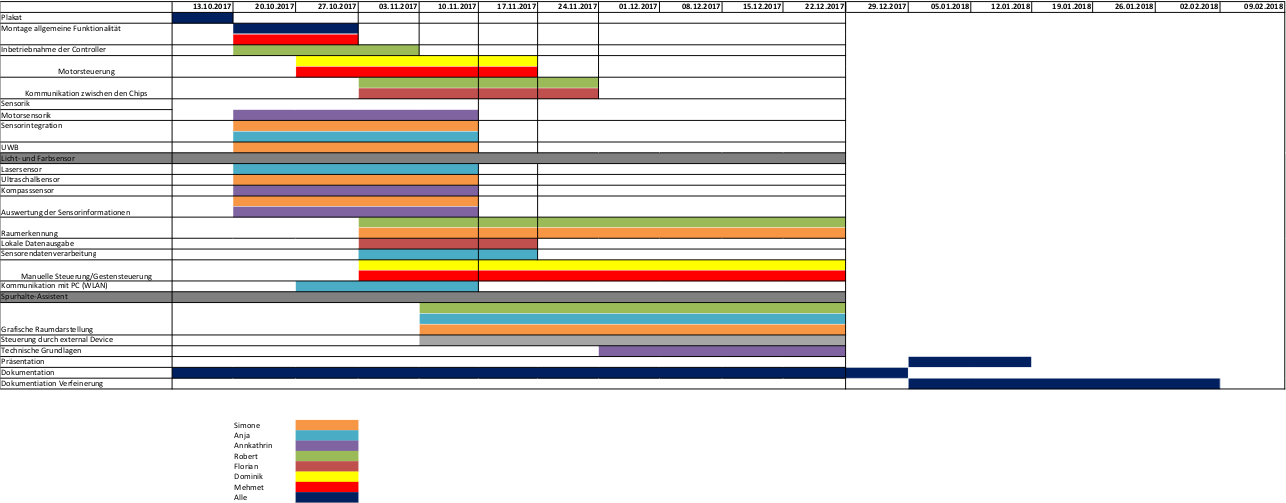
\includegraphics[width=200mm, height=130mm, scale=1]{Gantt_20_10.png}
	\caption{Gantt-Diagramm des erwarteten Projektverlaufs by Simone Huber}
	\label{fig:awesome_image}

\end{sidewaysfigure}

